\section{Question 4}
% \subsection{}
\paragraph{Consider a discrete dynamical system:
    $
        \begin{pmatrix}
            x_{i+1} \\
            y_{i+1} \\
            z_{i+1}
        \end{pmatrix} = A
        \begin{pmatrix}
            x_{i} \\
            y_{i} \\
            z_{i}
        \end{pmatrix}
    $.
    $$
        A=\begin{pmatrix}
            1.03552632  & 0.01842105 & -0.16447368 \\
            -0.00921053 & 1.10263158 & -0.00921053 \\
            -0.13815789 & 0.03947368 & 1.06184211
        \end{pmatrix}
    $$
}
\subsection{Caluclate the Next State}
\paragraph{If $(x_0,y_0,Z_0)=(100,100,100)$, caluclate $(x_1,y_1,z_1)$ and $(x_2,y_2,z_2)$}
\subsubsection{Analytics}
% 
$$$$
\begin{lstlisting}[style=pystyle]
import numpy as np

# Given matrix A
A = np.array([
    [1.03552632, 0.01842105, -0.16447368],
    [-0.00921053, 1.10263158, -0.00921053],
    [-0.13815789, 0.03947368, 1.06184211]
])

# Initial state (x0, y0, z0)
initial_state = np.array([100, 100, 100])

# Calculate the next states (x1, y1, z1) and (x2, y2, z2)
state_1 = np.dot(A, initial_state)
state_2 = np.dot(A, state_1)

# Print the results
print("Initial State:", initial_state)
print("Next State (x1, y1, z1):", state_1)
print("Next State (x2, y2, z2):", state_2)
\end{lstlisting}
% 
% 
% 
\subsubsection{Result}
\paragraph{Initial State: $[100\ 100\ 100]$ \\
    Next State (x1, y1, z1): $[ 88.947369\ 108.421052\ 96.31579 ]$ \\
    Next State (x2, y2, z2): $[ 78.26315889\ 117.84210399\ 94.26315877]$}
% 
% 
% 
% 
\subsection{Combination of Eigenvectors}
\paragraph{Given the initial state vector $(x_0, y_0, z_0)=(100, 100, 100)$, write this vector as a linear combination of eigenvectors of $A$.}
\subsubsection{Analytics}
% 
% 
% 
% 
% 
\paragraph{To express the initial state vector \((x_0, y_0, z_0) = (100, 100, 100)\) as a linear combination of the eigenvectors of matrix \(A\), we need to find the eigenvectors and eigenvalues of \(A\).}
% 
\paragraph{Let \(v_1, v_2, v_3\) be the eigenvectors of \(A\) corresponding to the eigenvalues \(\lambda_1, \lambda_2, \lambda_3\), respectively.}
% 
\paragraph{The expression for the initial state vector as a linear combination of eigenvectors is given by:}
% 
\paragraph{\[ \mathbf{x}_0 = c_1 \mathbf{v}_1 + c_2 \mathbf{v}_2 + c_3 \mathbf{v}_3 \]}
% 
\paragraph{where \(c_1, c_2, c_3\) are the coefficients to be determined.}
% 
\paragraph{Let's calculate the eigenvectors and eigenvalues using NumPy:}
% 
$$$$
% 
\begin{lstlisting}[style=pystyle]
import numpy as np

# Given matrix A
A = np.array([
    [1.03552632, 0.01842105, -0.16447368],
    [-0.00921053, 1.10263158, -0.00921053],
    [-0.13815789, 0.03947368, 1.06184211]
])

# Calculate eigenvectors and eigenvalues
eigenvalues, eigenvectors = np.linalg.eig(A)

# Given initial state vector
x0 = np.array([100, 100, 100])

# Solve for coefficients c1, c2, c3
coefficients = np.linalg.solve(eigenvectors, x0)

# Print the results
print("Eigenvectors:")
print(eigenvectors)
print("\nEigenvalues:")
print(eigenvalues)
print("\nInitial state vector as a linear combination of eigenvectors:")
print(f"x0 = {coefficients[0]:.2f} * v1 + {coefficients[1]:.2f} * v2 + {coefficients[2]:.2f} * v3")
\end{lstlisting}
% 
\paragraph{This code calculates the eigenvectors and eigenvalues of matrix \(A\) and then solves for the coefficients \(c_1, c_2, c_3\) in the expression \(\mathbf{x}_0 = c_1 \mathbf{v}_1 + c_2 \mathbf{v}_2 + c_3 \mathbf{v}_3\).}
% 

% % 
% % 
% \subsection{Gradient Descent from $(2, 4)$ for $F(x, y) = x^2 + y^2 - 6sin(x - y)$}
% % 
% % 
% % 
% \begin{lstlisting}[style=pystyle]
% import numpy as np
% import matplotlib.pyplot as plt
% import sympy as sp

% # Define symbolic variables
% x, y = sp.symbols('x y')

% # Define the function pandemic_model(x, y)
% F = x**2 + y**2 - 6*sp.sin(x - y)

% # Initialize the starting point
% x_current, y_current = 2, 4

% # Choose the step size parameter
% alpha = 0.1  # Change different values 0.1, 0.5, 1

% # Create lists to store the trajectory
% x_trajectory = [x_current]
% y_trajectory = [y_current]

% # Iterate for gradient descent
% for step in range(3):
%     # Calculate the gradient
%     gradient_x = sp.diff(F, x).subs({x: x_current, y: y_current})
%     gradient_y = sp.diff(F, y).subs({x: x_current, y: y_current})

%     # Update the point
%     x_current -= alpha * gradient_x
%     y_current -= alpha * gradient_y

%     # Add to the trajectory lists
%     x_trajectory.append(x_current)
%     y_trajectory.append(y_current)

% # Create a contour plot
% x_vals = np.linspace(-2, 4, 400)
% y_vals = np.linspace(-2, 6, 400)
% X, Y = np.meshgrid(x_vals, y_vals)
% Z = X**2 + Y**2 - 6*np.sin(X - Y)
% plt.contour(X, Y, Z, levels=50)
% plt.colorbar()

% plt.plot(x_trajectory, y_trajectory, marker='o', label='Gradient Descent Path')
% plt.xlabel('x')
% plt.ylabel('y')
% plt.title('Contour Plot of F(x, y) with Gradient Descent Path')
% plt.legend()
% plt.grid(True)
% plt.show()
% \end{lstlisting}
% % 
% % 

% \begin{multicols}{2} % 参数2表示创建两列布局
%     \begin{figure}[H]
%         \centering
%         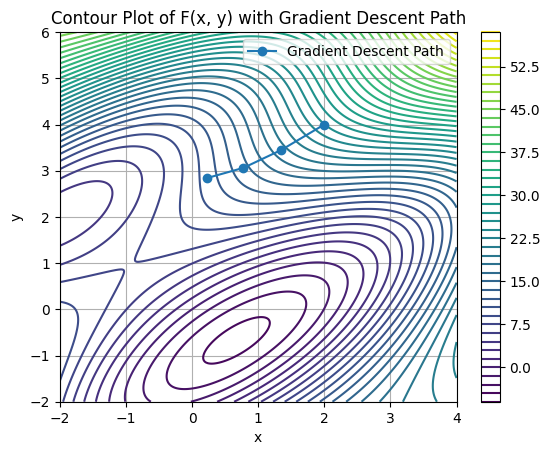
\includegraphics[width=0.5\textwidth]{pic/Gradient_Descent_Path_01.png}
%         \caption{step size parameter = 0.1}
%     \end{figure}
%     \columnbreak
%     \begin{figure}[H]
%         \centering
%         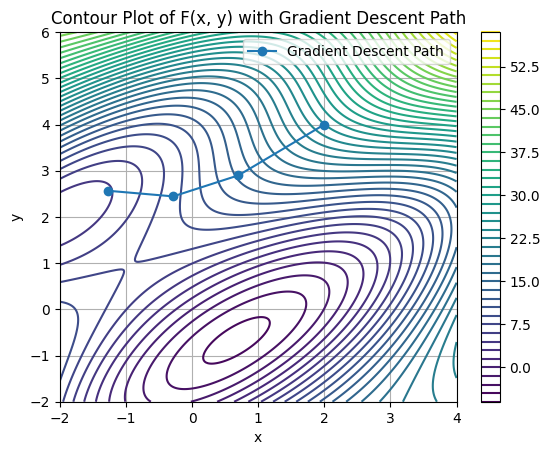
\includegraphics[width=0.5\textwidth]{pic/Gradient_Descent_Path_02.png}
%         \caption{step size parameter = 0.2}
%     \end{figure}
% \end{multicols}

% \begin{multicols}{2} % 参数2表示创建两列布局
%     \begin{figure}[H]
%         \centering
%         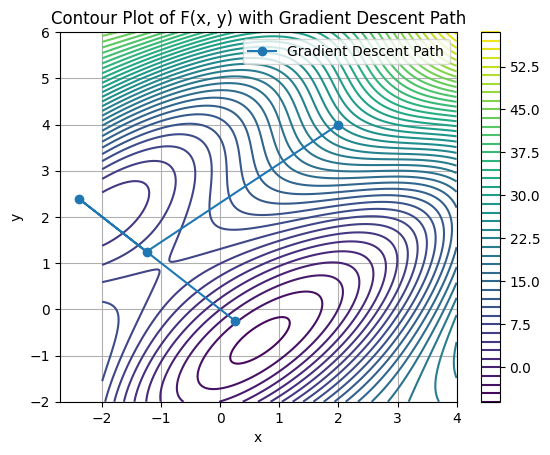
\includegraphics[width=0.5\textwidth]{pic/Gradient_Descent_Path_05.png}
%         \caption{step size parameter = 0.5}
%     \end{figure}
%     \columnbreak
%     \begin{figure}[H]
%         \centering
%         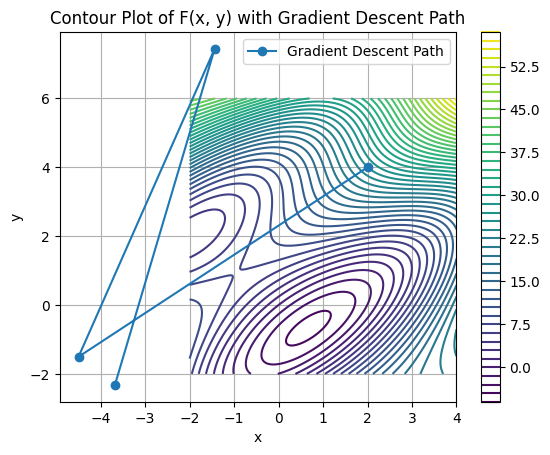
\includegraphics[width=0.5\textwidth]{pic/Gradient_Descent_Path_10.png}
%         \caption{step size parameter = 1.0}
%     \end{figure}
% \end{multicols}


% \subsection{Gradient Descent with more steps}
% \paragraph{\textbf{Analytics:}}
% \begin{enumerate}
%     \item Convergence to a Local Minimum: If the learning rate is chosen appropriately and the optimization problem is convex or has a single global minimum, gradient descent will converge to that minimum. may also be the global minimum.
%     \item Convergence to a Saddle Point: In non-convex optimization problems, gradient descent may converge to a saddle point rather than a local minimum. Saddle points are points where the gradient is zero, but they are not necessarily optimal. 
%     \item  Oscillation or Divergence: If the learning rate is too high, gradient descent may oscillate or even diverge. The model parameters may bounce back and forth, failing to converge. 
%     \item Slowing Down Near the Minimum: As gradient descent gets closer to the minimum, the step sizes become smaller because the gradient becomes smaller.
%     \item Flat Regions: In some optimization landscapes, there may be regions where the gradient is close to zero, but it is not a minimum. 
%     \item Longer Matplotlib Randering Time: when I set iteration number to 100, the plot is very complex, with a large number of data points, labels, and graphical elements, it can take longer to render (About 2.5 minutes). 
% \end{enumerate}

% % Gradient_Descent_Step_10
% \begin{figure}[H]
%     \centering
%     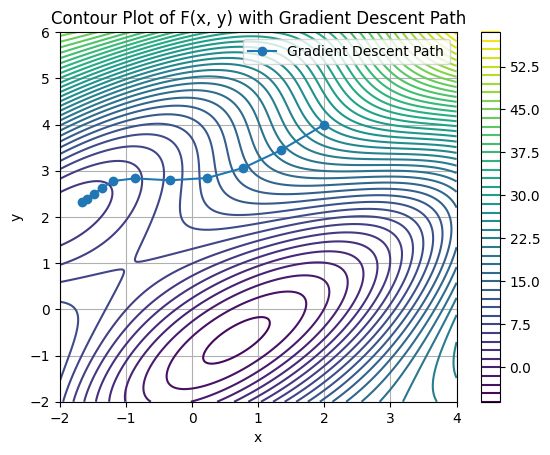
\includegraphics[width=0.75\textwidth]{pic/Gradient_Descent_Step_10.png}
%     \caption{Set iteration for 10 times, learning rate = 0.1}
% \end{figure}
% % 
% % 
% % 
% % 
% % 
% % 
% % 
% % 
% % 
% % 
% % 
% % 